\section{Global overview}

\begin{figure}[!ht]
	\centering
	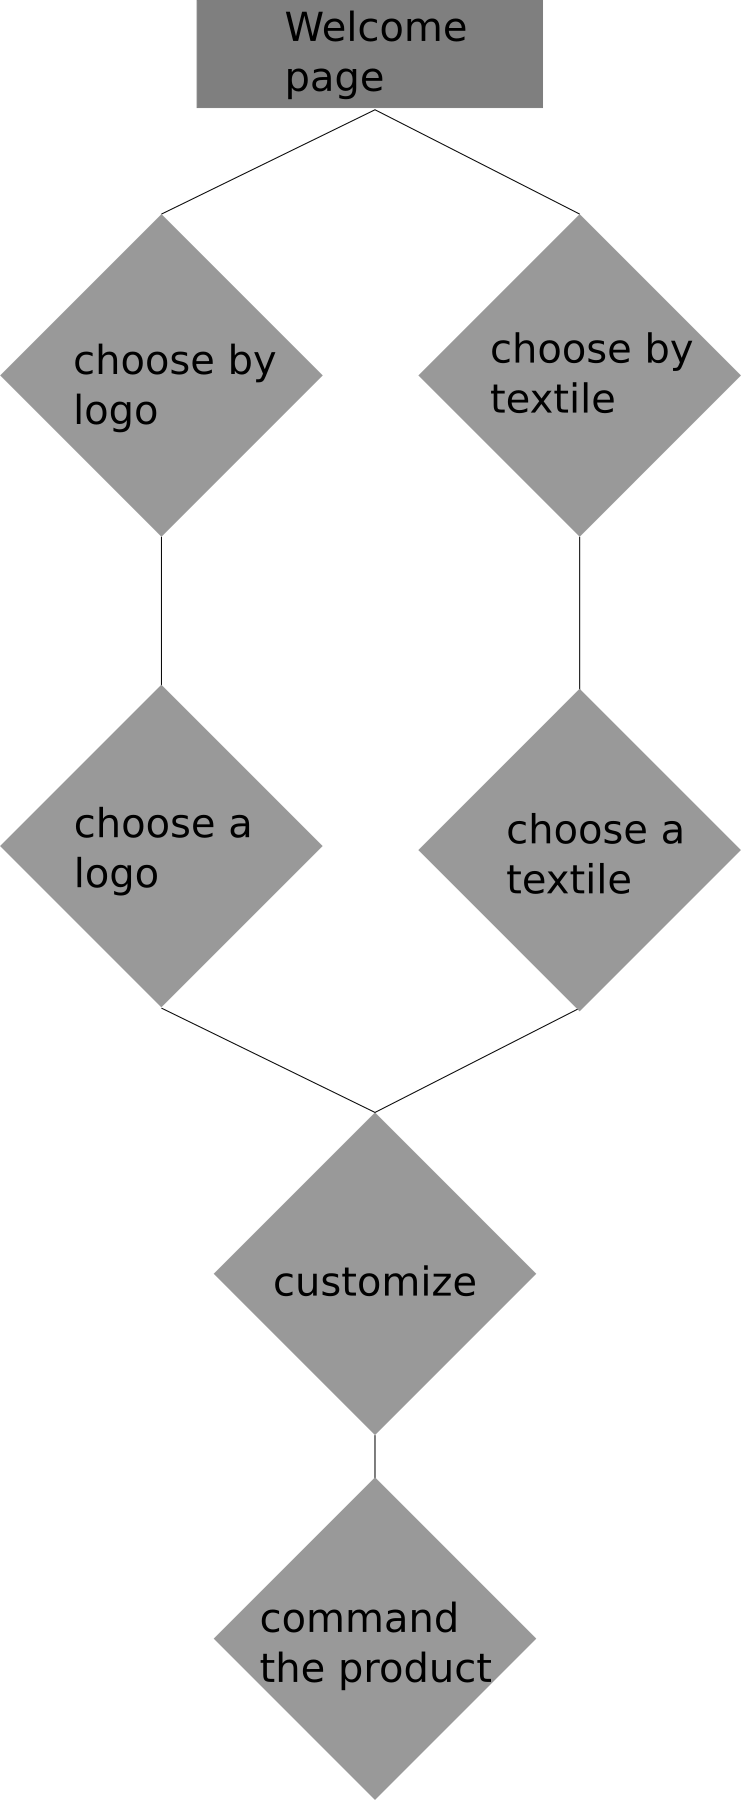
\includegraphics[width=0.2\textwidth]{overview/sellingProcess}
	\caption{Selling process of the website mycustom}
	\label{fig:sellingProcess}
\end{figure}

The selling process is represented on Figure \ref{fig:sellingProcess}. The idea is the following : the customer lands on the welcome page of mycustom. There, he can choose to browse the product either by textile or by logo. Once he has choose both, he can customize his choice, i.e move the logo on the textile, rotate the logo, increase the size of the logo, write text, change the color of the text ...

This is achieved by building the site in two distinct part. The first one is a single app page that allow the customer to browse the product as easily as possible. The seconde one is a graphical user interface (GUI) that allows the customer to customize his order. 

Note that some other part are add to the main page. One is so called the "collection éphémère" and its purpose is to promote the newest trends of the moment. This part is added at the beginning of the single app page.  An other one is added at the bottom of the single app page. It is the part "vendre" which purpose is to propose to the customer to signe in/up. A social network aspect needs to be implemented (it is currently not done). The idea behind this section of the main page is to propose the customer to sell his own logos and creations. Thus other customers can like logos, follow artistes ... 

Finally note that three search bars are added to the main page, one in the menu and two at the bottom of each choosing categories. These search bars are used to find specific textile/logos, thus adding an other way to choose a paire of textile-logo. 

